\documentclass[letterpaper]{article}
\usepackage{aaai}
\usepackage{times}
\usepackage{helvet}
\usepackage{courier}
\usepackage{amsmath,amsfonts,amssymb,amsthm}
\usepackage{array}
\usepackage{amsmath,amssymb}
%\usepackage{epsfig,subfigure}
\usepackage[vlined,algoruled,titlenumbered,noend]{algorithm2e}

\usepackage{graphicx}
\usepackage{caption}
\usepackage{subcaption}

\usepackage{verbatim}
%\usepackage{cite}

\frenchspacing

\newtheorem{lemma}{Lemma}
\newtheorem{assumption}[lemma]{Assumption}
\newtheorem{restr}{Restriction}   %[section]
\newtheorem{theorem}[lemma]{Theorem}
\newtheorem{proposition}[lemma]{Proposition}
\newtheorem{corollary}[lemma]{Corollary}
\newtheorem{hypothesis}[lemma]{Hypothesis}
\newtheorem{definition}[lemma]{Definition}

\usepackage[vlined,algoruled,titlenumbered,noend]{algorithm2e}
%\usepackage{proceed2e}

% If your paper is accepted and the title of your paper is very long,
% the style will print as headings an error message. Use the following
% command to supply a shorter title of your paper so that it can be
% used as headings.
%
%\runningtitle{I use this title instead because the last one was very long}

% If your paper is accepted and the number of authors is large, the
% style will print as headings an error message. Use the following
% command to supply a shorter version of the authors names so that
% they can be used as headings (for example, use only the surnames)
%
%\runningauthor{Surname 1, Surname 2, Surname 3, ...., Surname n}

%OLD
\newcommand{\fix}{\marginpar{FIX}}
\newcommand{\new}{\marginpar{NEW}}
\newcommand{\ind}[1]{\mathbb{I}[#1]}
\newcommand{\inde}{\mathbb{I}}

\newcommand{\var}{v}
\newcommand{\eq}{\leftarrow}

\newcommand{\LB}{\mathit{LB}}
\newcommand{\UB}{\mathit{UB}}

\newcommand{\B}{\mathbb{B}}
\newcommand{\E}{\mathbb{E}}
\newcommand{\I}{\mathbb{I}}
\newcommand{\R}{\mathbb{R}}

\newcommand{\F}{\mathbb{F}}
\renewcommand{\vec}[1]{\mathbf{#1}}

%NEW:
\newcommand{\tuple}[1] {\langle #1 \rangle}
\newcommand{\bvec}[1]{\textbf{#1}}
\newcommand{\indicator}{\mathbb{I}}%{I\!\!I}
\newcommand{\case}[2]{#2 &\text{ if } #1}%{#1 : #2}
\newcommand{\singlecase}[2]{#2 \quad \text{ if } #1}
\newcommand{\otherwise}[1]{#1 &\text{ otherwise}}
\newcommand{\pr}{p}
\newcommand{\nn}{0.16}


%%%%%%%%%%
% PDFINFO for PDFTEX
% Uncomment and complete the following for metadata if
% your paper is typeset using PDFTEX
% npdfinfof
\pdfinfo{
/Title (Symbolic Variable Elimination for Discrete and Continuous Graphical Models)
/Author (Scott Sanner and Ehsan Abbasnejad)
/Subject (Proceedings of the Twenty-sixth AAAI Conference (AAAI-12))
/Keywords (Graphical Models, Dynamic Programming, Hybrid Discrete and ContinuousProbabilistic Inference)
}
%%%%%%%%%%

\setcounter{secnumdepth}{0}  

\begin{document}

\title{Symbolic Gibbs Sampling in Piecewise Algebraic Graphical Models with Nonlinear Deterministic Constraints}
\author{
%Scott Sanner\\
%NICTA \& ANU\\
%Canberra, Australia\\
%{\tt ssanner@nicta.com.au}
%\And
%Ehsan Abbasnejad\\
%ANU \& NICTA\\
%Canberra, Australia\\
%{\tt ehsan.abbasnejad@anu.edu.au}
}

% TODO:
% - replace inference examples
% - emphasize oblique
% - add references to MTEs in Related Work... save .bbl
% - arbitrary expectations of polynomials?
% - computational complexity

\maketitle

\begin{abstract}
\begin{quote}
In many applications of probabilistic reasoning, there are deterministic relationships between
continuous random variables. These relationships create serious problems for approximate or exact inference.
%Such deterministic conditionals create serious problems for exact or approximate inference.
To avoid the complications, algorithms such as \emph{Bayesian inference using Gibbs sampling} (BUGS) simply disallow such dependencies.  
%For example, in BUGS it is impossible to model observed data that is the sum of two random variables. 
There are no known exact or Monte Carlo inference methods that can handle deterministic constraints beyond the limit of linear dependencies.
%Many classes of conjugate distributions %such as \emph{conditional linear Gaussians} 
%can handle linear deterministic conditionals. 
%General purpose full automated inference in the presence of non-linear deterministic constraints, however, is beyond the scope of the existing conjugate solutions and Monte Carlo algorithms.    
In this paper we fill this gap by contributing a novel framework which,
for the first time, carries out inference in models with nonlinear algebraic deterministic constraints. % that are not discussed in the literature so far.
Our second contribution is to provide an effective MCMC inference technique called \emph{Symbolic Gibbs}, based on the insight that in our model, most costly operations required for Gibbs sampling can be accomplished offline and prior to sampling. 
We evaluate this algorithm on models in physics and engineering and show that it is an order of magnitude faster than the baseline Gibbs sampler and a significant improvement over other Monte Carlo methods.  
\end{quote}
\end{abstract}

%\begin{abstract}
%\begin{quote} Many inference tasks require non-conjugate piecewise distributions. A recent line of research deals with classes of piecewise algebraic functions for which inference can be performed by means of symbolic methods. The current state-of-the-art such class is the family of piecewise polynomials with linear constraints. In this work, we vastly generalize this class to cover piecewise functions in which the partitioning constraints and the function values in each partition are both in the form of fractions of multivariate polynomials. We show that for this class, by combining Gibbs sampling with symbolic methods, a high performance black box sampling techniques can be achieved. The key insight is that in this class, cumulative distribution functions required for Gibbs sampling can be computed prior to sampling, symbolically and in closed form. Apart from expressiveness, the afore mentioned class of piecewise functions is reach enough to handle sophisticated algebraic deterministic dependencies among the random variables. \end{quote}
%\end{abstract}


%The authors describe a new methodology for frequency and duration (F&D) assessment in composite generation and transmission reliability evaluation. The proposed approach uses the concept of conditional probability to characterize the contribution of each component to the frequency indices, and allows the calculation of F&D indices at both system and bus level. The algorithm is easy to implement, and requires the same computational effort as the estimation of the system loss of load probability (LOLP) and the system expected power not supplied (EPNS) indices. Case studies with utility-derived systems are presented and discussed

\section{Introduction}
\label{sec:intro}
Graphical models (GMs) are the lingua franca for probabilistic reasoning.
They denote the conditional dependence structure between random variables by directed or undirected graphs \cite{koller2009probabilistic}. A (random) variable is deterministic if its conditional distributions have zero variances. 
%Unobserved deterministic random variables that is, variables that cannot be given data or initial values (corresponding to \emph{logical nodes} in BUGS software) almost only provide notational convenience.
Observed deterministic variables represent deterministic dependencies on other variables.
Such constraints can appear in a variety of real-world applications.
For instance, 
such deterministic relationships between random variables might be governed by natural laws 
(such as Kirchhoff's circuit laws or Newtonian mechanics).

To motivate the discussion consider the following concrete example:  
%%%%%%%%%%%%%%%%%%%%%%%%%%%%%%%%%%%%%%%%%%%%%%%%%%%%%%%%%%%%%%%%%%%%%%%%%%
\begin{figure}
\begin{center}
%\begin{minipage}{1\linewidth}
\begin{center}
%\vspace{-1mm}
\quad
\begin{subfigure}{0.19\linewidth}
                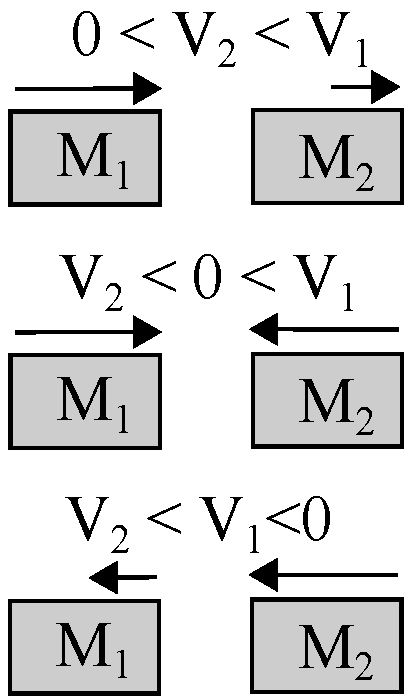
\includegraphics[width=1\linewidth]{Figs/little-momentum0.pdf}
                \caption{}
                \label{fig:mom0}
        \end{subfigure}%
\qquad
\begin{subfigure}{0.52\linewidth}
                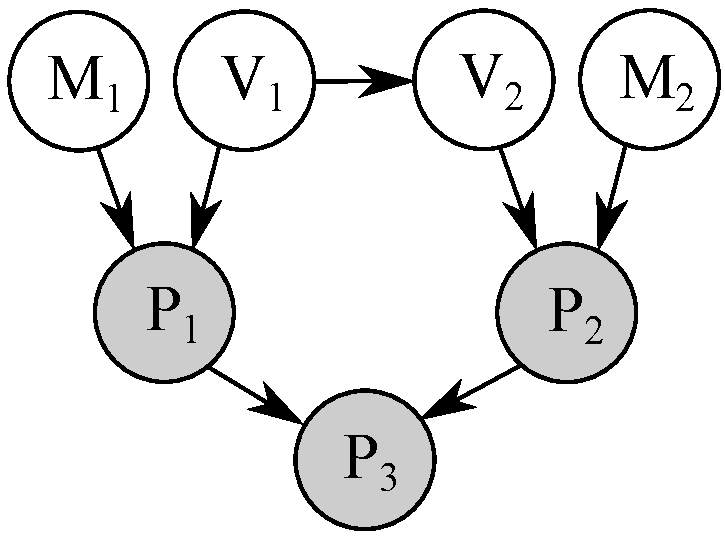
\includegraphics[width=0.80\linewidth]{Figs/little-momentum1.pdf}
                \caption{}
                \label{fig:mom00}
        \end{subfigure}%
\end{center}
\vspace{-1mm}
\caption{\footnotesize 
Collision of masses $M_1$ and $M_2$ with velocities $V_1$ and $V_2$ and momenta $P_1$ and $P_2$. 
(a) Collision happens if and only if $V_1>V_2$. (b) Corresponding Bayesian network. The non-filled and filled Filled circles represent stochastic and deterministic random variables respectively.} 
\label{fig:mom2}
\vspace{-4mm}
%\end{minipage}
\end{center}
\end{figure}

%%%%%%%%%%%%%%%%%%%%%%%%%%%%%%%%%%%%%%%%%%%%%%%%%%%%%%%%%%%%%%%%%%%%%%%%%%
%\vspace{1mm}\\
{\bf Example (Collision). }
\emph{Masses $M_1$ and $M_2$ with velocities $V_1$ and $V_2$ (and consequently momenta $P_1 = M_1 V_1$ and $P_2 = M_2 V_2$) collide to form a single mass ($M_1 + M_2$) with momentum $P_3 = P_1 + P_2$ (assuming that there is no dissipation).
Masses and velocities are unknown but 
their prior distributions are given as follows (note that as Figure~\ref{fig:mom0} shows, a collision only happens if $V_2 < V_1$):  
}%end \emph
{\footnotesize
\begin{align*}
&M_1 \sim \mathcal{U}(0.1, \, 2.1) 
&&M_2 \sim \mathcal{U}(0.1, \, 2.1)
\\
&V_1 \sim \mathcal{U}(-2, \, 2)
&&V_2 \sim \mathcal{U}(-2, \, V_1)
\end{align*} 
\emph{
The conditional dependencies of these random variables are illustrated in 
Figure~\ref{fig:mom00}.
Conditioned on the observation $P_3 = 3$, the posterior joint distribution of $M_1$, $M_2$, $V_1$ and $V_2$ is desired. 
} %\emph
}


In this example, the deterministic constraint is: 
{\footnotesize
\begin{equation}
\label{eq:moment-constraint}
P_3 = P_1 + P_2 = M_1 V_1 + M_2 V_2 = 3
\end{equation}
and corresponds to the 0-variance conditional distribution: 
$$
\pr(P_3 \,|\, M_1, V_1, M_2, V_2) = \delta[P_3 - (M_1 V_1 + M_2 V_2)] = 3
$$
}
Unfortunately, 
beyond the limit of linear relationships, such as $Z = X_1 + X_2$, 
current probabilistic inference systems cannot handle deterministic constraints.
BUGS \cite{lunn2009bugs}, the popular software for analysis of statistical models, 
totally disallows deterministic relationships between continuous random variables.

Families of distributions such as \emph{conditional linear Gaussians (CLG)} \cite{lauritzen2001stable}
allow linear deterministic constraints but as mentioned, inference in the presence of nonlinear deterministic constraints on continuous random variables is still an open problem.

In this paper we solve this problem for a large class of nonlinear multivariate algebraic deterministic constraints in the form of polynomial fractions. 
Our main contributions are:
\begin{itemize}
\item Introducing  an expressive class of functions 
(called PPPFs for \emph{Polynomial-Piecewise Polynomial Fractions}) that facilitates inference in the presence of  linear/nonlinear algebraic deterministic constraints.
\item Presenting an efficient inference method (called \emph{Symbolic Gibbs}) that matches well with the provided model and handles deterministic constraints.  
\end{itemize}

%The proposed class if expressive functions includes 
%Our first contribution is to propose an extremely expressive class of functions for inference in graphical %models (such as Bayesian networks, Markov random fields, etc.).
PPPFs are piecewise polynomial fractions where the variable space is partitioned by polynomial inequalities.
%To show the importance of fractional functions we note that %and nonlinear partitions we note that 
The key insight is that the algebraic constraints preserved PPPF form after collapsing which immediately extends the application of PPPFs to models with sophisticated deterministic algebraic constraints. 
We note that 
even in simple models such as \emph{collision example}, distributions can be piecewise fractional. 
For example:  
\[
\pr(V_2 \,|\, V_1) = \mathcal{U}(-2, V_1)
=
\begin{cases}
  \case{\scriptstyle (V_2 > -2), \, (V_2 < V_1)}{\frac{1}{V_1 + 2}}\\
 \otherwise{0}
 \end{cases}
\]

To show the critical role of nonlinear partitioning conditions in handling the algebraic deterministic constraints, 
let us solve equation~\ref{eq:moment-constraint} for a variable (e.g.\ $V_2$):
$V_2 = \frac{3 - M_1 V_1}{M_2}$) and modify $\pr(V_2 \,|\, V_1)$ by substituting $V_2$ with its the solution.
We will see that this substitution leads to $\pr(V_2 \,|\, V_1, P_3 = 3)$:
\begin{equation}
\label{e:fractional-constraint}
\begin{cases}
  \case{(\frac{3 - M_1 V_1}{M_2} > -2) , \, (\frac{3 - M_1 V_1}{M_2} < V_1)}{\frac{1}{V_1 +2}}\\
  \otherwise{0}
  \end{cases}
\end{equation}
Clearly, this transformation has created a piecewise function with non-linear partitioning conditions.

Recently, piecewise polynomials have attracted attention.
So far, piecewise polynomials with hyperrectangular, hyper-rhombus and linear partitioning constraints have been used in Bayesian networks \cite{shenoy2011inference,shenoy2012two,Sanner:12}.
%hyperrectangular-piecewise polynomials \cite{shenoy2011inference,shenoy2012two,Sanner:12},
%hyper-rhombus-piecewise polynomials \cite{shenoy2012two} and the most general so far, linear-piecewise polynomials \cite{Sanner:12} have been used for inference in Bayesian networks.\footnote{ By \emph{A-piecewise B} we refer to piecewise functions where the function value in each partition is in class \emph{B} and the conditions partitioning the space of variables are (conjunctions of functions) in class \emph{A}.}
These models can only handle linear dependencies and 
our model is more expressive than all of them. 
%This, for the first time, enables probabilistic inference be carried on a large domain of interesting and new  applications.  

The second contribution, as mentioned, is a new variation of Gibbs sampling.  
Gibbs samplers are robust in the sense that they do not need any parameter tuning.
However, they are computationally expensive since to take a single sample they require to compute many univariate integrals (to generate the CDFs of conditional distributions).
We notice that a large subset of PPPFs have closed form (symbolic) integrals. 
The idea of Symbolic Gibbs is to compute a single analytic integral for each variable by keeping the remaining variables uninstantiated. 
The actual process of CDF computation per sample  
simply involves instantiation of the already computed CDFs rather than computing them on the fly.
This dramatically decreases the amount of necessary computations and as our experimental results show, it improves the performance significantly.

In the following sections after a brief introduction to Graphical models, 
followed by an algorithm for inference in the presence of deterministic constraints.
We then explain the restrictions of PPPFs, compare our method with other samplers and conclude. 

\section{Graphical Models (GMs)}
Let $\vec{X} = \{X_1, X_2, \ldots\}$ be a set of random variables with realizations in the form 
$\vec{x} = \{x_1, x_2, \ldots\}$.\footnote{
As a common abuse of notation, in case there is no ambiguity, we do not distinguish between random variables and their realizations; e.g., we abbreviate $\pr(X_i = x_i)$ with $\pr(x_i)$.}
$\vec{X}$ may contain discrete and continuous variables. 
However, for the sake of notational consistency, %and since the problems tackled in this paper only hold for continuous variables, 
we only consider continuous models throughout. 
Note that inference in presence of discrete deterministic constraints is trivial.
Therefore, generalization of the presented framework to hybrid discrete/continuous models is straightforward.   

To cover both directed and undirected graphical models we use
\emph{factor graph} notation \cite{kschischang2001factor}
and represent a joint probability distribution $\pr(\vec{X})$ in a factorized form as follows: 
\begin{equation}
\label{e:factor-graph}
\pr(\vec{X}) = \frac{1}{C} \prod_{\Psi \in \boldsymbol\Psi} \Psi (\vec{X})
\end{equation}
where 
$\Psi(\vec{X})$ is a non-negative, real-valued potential function (of a subset of $\vec{X}$) and $C$ is a (not necessarily known) normalization constant.
%The inference procedure that will be presented does not require the normalization constant be known. 

If the valuation of variables $\bvec{E} \subset \bvec{X}$ is observed,
the joint probability of the remained variables $\bvec{X} \backslash \bvec{E}$ conditioned on the observation ($\bvec{E} = \bvec{e}$) is simply proportional to $\pr(\bvec{X})$ in which $\bvec{E}$ is instantiated by $\bvec{e}$:
\begin{equation}
\label{e:posterior-joint}
\pr_{\bvec{e}}(\bvec{X} \backslash \bvec{E}) := 
\pr(\bvec{X} \backslash \bvec{E} \,|\, \bvec{e}) \propto 
\pr(\bvec{X} \backslash \bvec{E}, \bvec{E} = \bvec{e}) \propto
\prod_{\Psi \in \boldsymbol\Psi} \Psi (\vec{X})|_{\bvec{E} \leftarrow \bvec{e}}
\end{equation}
Provided with (non-normalized) $\pr_{\bvec{e}}(\cdot)$ with dimensionality reduced from $|\bvec{X}|$ to $|\bvec{X}| - |\bvec{E}|$, probabilistic inference is facilitated. 
For example, 
the \emph{posterior} probability of \emph{query} variables $\vec{Q} \subset \vec{X}$ 
%given \emph{evidence} variables $\vec{e} \subset \vec{x}$ 
is computed by marginalizing variables that are not in the query or evidence,
$\{W_1, \ldots, W_k\} := \vec{X} \backslash (\vec{Q} \cup \vec{E})$:
\begin{equation}
\label{e:inference}
\pr(\vec{Q} \,|\, \vec{e}) \propto 
\int_{w_1 = -\infty}^{\infty} \!\!\!\!\!\! \cdots \int_{w_k = -\infty}^{\infty}
%\prod_{\Psi \in \boldsymbol\Psi} \Psi(\vec{x})
\!\!\!\!\!\!\!\! \pr_{\bvec{e}}(\bvec{Q}, w_1, \ldots, w_k )
\, d_{w_1} \ldots d_{w_k}
\end{equation}
%We will shortly show that unlike the conventional graphical models, in models with deterministic constraints, the creation of joint distribution of unobserved variables requires more computations. We first formalize such models. 
\subsection{Inference in GMs}
\textbf{Closed form inference.}
The main challenge for closed inference is the computation of multiple integrals required for marginalization (equation~\ref{e:inference}).
There are a few classes of functions which are closed under integration.
However, none of these classes can handle deterministic constraints beyond the level of linear constraints.
\\
\textbf{Monte Carlo methods}
%An alternative to exact inference is to approximate the joint distribution by a set of samples drawn from it using Monte Carlo methods. By the law of large numbers, this approximation is asymptotically unbiased. Using samples, the costly marginalization operation is avoided since the conditional probability $\pr(\bvec{q} \,| \, \bvec{e})$ is simply approximated by the number of samples satisfying $\bvec{q} \cap \bvec{e}$ divided by the number of samples satisfying $\bvec{e}$.
%Note that unlike other approximate methods, inference via sampling leads to asymptotically unbiased solutions i.e.\ by taking sufficient number of samples, the \emph{posterior} can be approximated by an arbitrary precision.
Approximating the posterior distribution via drawing samples from it by Monte Carlo methods 
provides an asymptotically unbiased tool that completely avoids the hassle of multiple integrations required in closed-form sampling.   
Three major such methods are as follows:

\emph{Rejection sampling}: In this method, to draw a sample from 
a distribution $p(\bvec{X})$, a sample $\bvec{x}$ is taken from another distribution $q(\bvec{X})$
such that $p(\bvec{X})/q(\bvec{X})$ is bound by a known constant $c$
and samples can be taken from $q(\bvec{X})$ efficiently.
The produced sample is accepted with probability $p(\bvec{x}) / c q(\bvec{x})$, 
otherwise it is rejected and the process is repeated. 

\emph{Metropolis-Hastings (MH)}:
To draw a new sample $\bvec{x}^{(t)}$ from a distribution $p(\bvec{X})$, given a previously taken sample $\bvec{x}^{(t-1)}$, 
MH takes a sample $\bvec{x}'$ from a symmetric \emph{proposal density} $q(\bvec{X} |\, \bvec{x}^{(t-1)})$. 
%from which samples can be taken efficiently 
%(often an isotropic \emph{Gaussian} centered at $\bvec{x}^{(t-1)}$). 
With probability $\min \big(1, p(\bvec{x}')/p(\bvec{x}^{(t-1)}) \big)$, 
$\bvec{x}'$ is accepted as the next sample ($\bvec{x}^{(t)} \leftarrow \bvec{x}'$), otherwise, $\bvec{x}^{(t)} \leftarrow \bvec{x}^{(t-1)}$. 
Choosing a good \emph{proposal} is problem-dependent and requires tuning. 


\emph{Gibbs sampling}:
Gibbs is a robust sampling tool in the sense that it does not require known bounds, tuned proposal densities or parameters.
Drawing a sample for $\bvec{X} = (X_1, \ldots, X_N)$ takes place in $N$ steps.
In the $i$-th step, $X_i$ is sampled conditioned on the last realization of the others:
$x_i \sim \pr(X_i \,|\, \bvec{x}_{-i})$. 
To perform this task, the following univariate \emph{Cumulative Distribution Function} (CDF)
is computed by equation~(\ref{e:cdf}) and samples are taken by inverse transform sampling. 
{\footnotesize
\begin{equation}
\label{e:cdf}
F(X_i  \,|\, \bvec{x}_{-i}) 
\propto
\int_{-\infty}^{X_i} \!\!\!\! \pr(X_i = t, \bvec{x}_{-i}) \, d  t
\end{equation} 
}
%Computation of $N$ univariate integrals per sample is costly and this makes Gibbs sampling a relatively slow sampler. However, we will show that the family of PPPF functions, the performance of Gibbs sampling can be improved significantly.

In the next section, we formalize GMs with deterministic variables. 

\section{Graphical Models with Deterministic Constraints}
Consider a graphical model with random variables $\bvec{X} := \bvec{Y} \cup \bvec{Z}$
where $\bvec{Y}$ and $\bvec{Z}$ are respectively called \emph{stochastic} and \emph{deterministic}  variables.
In the network specification, for each deterministic variable $Z \in \bvec{Z}$ there exists exactly one \emph{associated potential function }
$\Psi_Z := \delta[Z - G^Z]$ (indicating the deterministic dependency $Z = G^Z$)
where $\delta[\cdot]$ is \emph{Dirac delta} function and $G^Z$, the \emph{logical value} of $Z$,  is an expression that does not involve $Z$ (i.e.\ $Z \not\in \textsc{Scope}(G^{Z})$).\footnote{
As an instance, in the \emph{collision example}, $G^{P_1} = M_1 V_1$.
}
Finally, the following restriction guarantees that the deterministic variables are not defined recursively:
\begin{equation*}
\forall Z, Z' \in \bvec{Z} \qquad Z \in \textsc{Scope}(G^{Z'}) \Rightarrow Z' \not\in \textsc{Scope}(G^Z)
\end{equation*}
The set of all potentials $\boldsymbol{\Psi} := \boldsymbol{\Psi^D} \cup \boldsymbol{\Psi^S}$
where
$\boldsymbol{\Psi^D} :=\{\Psi_Z \,|\, Z \in \bvec{Z}\}$ is the set of deterministic potentials
and $\boldsymbol{\Psi^S}$ is the set of stochastic (i.e.\ conventional) potentials. 

In the next sections, inference and its limitations in GMs with deterministic random variables are studied.
%%%%%%%%%%%%%%%%%%%%%%%%%%%%%%%%%%%%%%%%%%%%%%%%%%%%%%%%%%%%%%%%%
\incmargin{0.5em}
%\SetInd{0.5em}{1em}
\begin{algorithm}[hb!]
\SetKwInOut{Input}{input}
\SetKwInOut{Output}{output}
\dontprintsemicolon
{\small
\Input{
$\mathbb{E} = \{\tuple{E_i, e_i}\}_i$ 
// \emph{\small evidence}\\
%$\bvec{Z} = \{Z\}$, deterministic variables\\
$\boldsymbol{\Psi} = \boldsymbol{\Psi^D} \cup \boldsymbol{\Psi^S}$ 
 //\emph{set of potentials.
 } }
\Output{posterior joint distribution of a subset of variables from which, all other variables can be decided.}
\BlankLine
{
\Begin{
	//\emph{{\bf \sc Step 1.} Instantiation of the observed variables:}\\  
	\ForAll{$\tuple{E, e} \in \mathbb{E}$}
	{
		\textbf{forall }{$\Psi \in \boldsymbol{\Psi}$} \textbf{ do } {$\Psi \leftarrow \Psi|_{E \leftarrow e}$	}
	}
	\textbf{end for}\\
 \vspace{1mm}
	//\emph{{\bf \sc Step 2.} Isolating deterministic variables:}\\  
	\ForAll{$\Psi_Z = \delta [Z - G^Z] \in \boldsymbol{\Psi^D}$}
	{
		\textbf{forall }{$\Psi \in \boldsymbol{\Psi}$} \textbf{ do } 
		{$\Psi \leftarrow \Psi|_{Z \leftarrow G^Z}$	}
	}
	\textbf{end for}\\
 \vspace{1mm}
	//\emph{{\bf \sc Step 3.} Joint factor formation:}\\  
	$\pr_{\bvec{e}} \leftarrow \prod_{\Psi \in \boldsymbol{\Psi^S}} \Psi$\\
     %$J \leftarrow 1$\\
	%\ForAll{$\Psi \in {\boldsymbol\Psi}^{S}$}
	%{
	%	$J \leftarrow J \otimes \Psi$
	%}
	%\textbf{end for}\\
 \vspace{1mm}
	//\emph{{\bf \sc Step 4.} Collapsing determinism:}\\  
	\ForAll{$\tuple{E, e} \in \mathbb{E}$ \textbf{\emph{such that}} $E \in \bvec{Z}$}
	{
		\textbf{let} $\tuple{Y, G^Y} = \textsc{solve}(G^E=e)$ //  \emph{assuming that a unique solution exists.}\\
		$\pr_{\bvec{e}} \leftarrow \pr_{\bvec{e}}|_{Y \leftarrow G^Y}$ 
	// \emph{substituting $Y$ with its solution}\\	
	}
	\textbf{end for}\\
\Return{$\pr_{\bvec{e}}$}\;
}
}%end small
}
\caption{{\sc PosteriorJoint}  \label{alg:posterior-joint}}
\end{algorithm}
\decmargin{0.5em}
%%%%%%%%%%%%%%%%%%%%%%%%%%%%%%%%%%%%%%%%%%%%%%%%%%%%%%%%%%%%%%%%%

\section{Inference in GMs with Deterministic Constraints}
We allow both stochastic and deterministic variables to be observed by evidence.  
We are interested in deterministic variables with associated logical values  
created by the plus, multiplication, minus, division operations and therefore 
are in the form of fractions of polynomials.

In order to conduct inference we should first compute 
the posterior joint distribution  
(as in equation~\ref{e:posterior-joint}).
To perform this task, we propose \emph{collapsing} (i.e.\ marginalizing over) all observed and non-observed deterministic variables. The details are presented in the next subsection. 

Provided with the posterior, the main task of inference is carried out by equation~(\ref{e:inference}).
For this task we will rely on Symbolic Gibbs sampling.

\subsection{Posteriors in GMs with Deterministic Constraints}

The aim of this section is to find a posterior joint distribution over a subset $\bvec{X}'$ of $\bvec{X}$
such that any other variable (either stochastic or deterministic)
can be expressed as a function of $\bvec{X}'$.
The procedure, as formalized in Algorithm~\ref{alg:posterior-joint}, is as follows: 
\begin{enumerate}
\item \emph{Instantiation of observed variables.} In all potentials, stochastic observed variables are instantiated
(like the instantiation $\bvec{E} \leftarrow \bvec{e}$ in equation~\ref{e:posterior-joint}).
%
\item \emph{Isolating deterministic variables.} In all potentials, all deterministic variables $Z$, are 
substituted with their associated logical value $G^Z$ (so, the potential $\delta[x - G^x]$ itself is replaced by 1). Note that by the definition of Dirac $\delta$, this simply means all deterministic variables are marginalized.
%
\item \emph{Joint factor formation.} the product of the remaining potentials is computed (as in equation~\ref{e:posterior-joint}).   
%
\item \emph{Collapsing determinism.} 
What remains is to condition on the deterministic constraints.
For each deterministic constraint $Z = c$ (where $c$ is a constant),
$(G^Z = c)$ is solved w.r.t.\ some variable $Y \in \textsc{Scope}(G^Z)$ (assuming that it is solvable with a single solution w.r.t.\ at least one such variable).
Subsequently, in all potentials, $Y$ is substituted by its solution (called $G^Y$).\footnote{For instance in the \emph{collision example}, 
$\textsc{solve}\big((M_1 V_1 + M_2 V_2)=3 \big)$ can be $\tuple{V_2, \frac{3 - M_1 V_1}{M_2}}$.} 
%
\end{enumerate}
%The output of this algorithm is a non normalized joint distribution of  a subset of none-deterministic variables. Provided with this joint, the marginal distribution of all query variables (either probabilistic or deterministic) can be computed by means of sampling as will be discussed later.

%Note that these operations alter the normalization constant and the resulting function is only proportional to the corresponding joint distribution. However, most inference algorithms do not require normalization.Some of these algorithms are provided in the next section. However, prior to that we discuss the limitations of Algorithm~\ref{alg:posterior-joint} 
The family of deterministic constraints studied in this work includes polynomial fractions.
For this family, 
the unique solution assumption (required in Step 4 of Algorithm~\ref{alg:posterior-joint})
in general holds if $G^Z$, the logical values of deterministic variables, are linear w.r.t. some variables.
That is, for some variable $Y$, $G^Z$ can be stated as: 
{\footnotesize
\begin{equation}
\label{eq:evidence-form}
G^Z = \frac{\mathcal{A} \cdot Y + \mathcal{B}}{\mathcal{C} \cdot Y + \mathcal{D}}
\end{equation}
}
where $\mathcal{A}$ to $\mathcal{D}$ are constant or univariate/multivariate polynomials and $Y$ is not in their scopes.


\subsection{Symbolic Gibbs Sampling}
Our symbolic Gibbs sampling is based on a simple but significantly useful insight.
Namely, if the multivariate function $\pr(X_1, \ldots, X_N)$
has an analytic (symbolic) integral for all its variables $X_i$,
then, instead of using equation~\ref{e:cdf}, we map each variable $X_i$ to its corresponding symbolic CDF: 
{\footnotesize
\begin{equation}
\label{e:cdf-symbolic}
F(X_i  \,|\, \bvec{X}_{-i}) 
\propto
\int_{-\infty}^{X_i} \!\!\!\!\! \pr(X_i = t , \bvec{X}_{-i}) \, d  t
\end{equation} 
}
Note that the difference between (\ref{e:cdf}) and (\ref{e:cdf-symbolic}) is that in the former, 
all variables except $X_i$ are already instantiated therefore 
$F(X_i  \,|\, \bvec{x}_{-i})$ is a univariate function but in  (\ref{e:cdf-symbolic}), 
although variables $\bvec{X}_{-i}$ are treated as constants but they are kept uninstantiated and symbolic.
As a result, $F(X_i \,|\, \bvec{X}_{-i})$ is a multivariate analytic function. 
%as Algorithm~\ref{alg:analytic-cdf} shows, 
%we can create a map from variables $X_i$ to their corresponding closed-form CDFs.

The map (called {\sc VarToCDF}) from variables $X_i$ to their symbolic CDFs
$F(X_i \,|\, \bvec{X}_{-i})$ is passed to the main symbolic Gibbs sampling procedure in Algorithm~\ref{alg:symbolic-gibbs}.
During the sampling process, 
to sample $x_i \sim \pr(X_i \,|\, \bvec{x}_{-i})$
it is sufficient to get the (multivariate) symbolic CDF associated to $X_i$ from the map
and instantiate it with $\bvec{x}_{-i}$ to obtain the appropriate univariate CDF.

By this method, instead of computing $N \times T$ integrals for $T$ samples, only $N$ integrals are computed and 
$N \times T$ function instantiations are performed. But function instantiation is much faster than integration.
Therefore, the algorithm leads to a major improvement in speed.

What remains is to show that a large subset of PPPF functions indeed have closed-form integrals. 

%\begin{equation*}
%\int_{X_i= -\infty}^{x_i} \!\!\!\!\!\!\!\!\!\! \pr(X_1, \ldots, X_N) \, d  X_i
%\end{equation*} 
\begin{comment}
%%%%%%%%%%%%%%%%%%%%%%%%%%%%%%%%%%%%%%%%%%%%%%%%%%%%%%%%%%%%%%%%%
\incmargin{-0.3em}
\SetInd{0.1em}{0.6em}
%\linesnumberedhidden
% \linesnumbered
\begin{algorithm}[hb!]
%\SetKwFunction{eliminate}{{\sc Eliminate}}
\SetKwInOut{Input}{input}
\SetKwInOut{Output}{output}
\dontprintsemicolon
{\small
\Input{$\pr(\bvec{X})$ // \emph{\small joint distribution of variables $\tuple{X_1, \ldots, X_N}$.} }
\Output{{\sc VarToCDF}: $\bvec{X} \rightarrow (\bvec{X} \rightarrow \mathbb{R})$ // \emph{\small a map from variables to their non-normalized analytical CDFs. }}
\BlankLine
{\small
\Begin{   
   {\sc VarToCDF} = an empty map\\
   \ForEach{$X_i \in \bvec{X}$}{
//\emph{non-normalized analytical CDF w.r.t.\ $X_i$:}\\
	$F_i(\bvec{X}) := \int_{v = -\infty}^{X_i} \pr(X_1, \ldots, X_{i-1}, v, X_{i+1}, \ldots, X_N) dv$\\ 
     {\sc VarToCDF}.put($X_i$, $F_i(\bvec{X})$)
   	}
	\textbf{end for}   \\
   \Return{\sc VarToCDF}\;
}
}%end small
}
\caption{{\sc AnalyticCDF}  \label{alg:analytic-cdf}}
\end{algorithm}
\decmargin{-0.3em}
%%%%%%%%%%%%%%%%%%%%%%%%%%%%%%%%%%%%%%%%%%%%%%%%%%%%%%%%%%%%%%%%%
\end{comment}
%%%%%%%%%%%%%%%%%%%%%%%%%%%%%%%%%%%%%%%%%%%%%%%%%%%%%%%%%%%%%%%%%
\incmargin{-0.5em}
\SetInd{0.1em}{0.7em}
%\linesnumberedhidden
% \linesnumbered
\linesnotnumbered
\begin{algorithm}[hb!]
%\SetKwFunction{eliminate}{{\sc Eliminate}}
\SetKwInOut{Input}{input}
\SetKwInOut{Output}{output}
\dontprintsemicolon
{\small
\Input{$\bvec{X} := \tuple{X_1, \ldots, X_N}$, // \emph{\small random variables} \\
 $\bvec{x}^{(0)} := \tuple{x_1^{(0)}, \ldots, x_N^{(0)}}$, // \emph{\small initial values} \\
{\sc VarToCDF}, //\emph{\small variables to analytic CDFs map} \\
 $T$ // \emph{\small number of desired samples } }
\Output{list of taken samples}
\BlankLine
{\small
\Begin{   
   \ForAll{$t= 1, 2, \ldots T$}{
	$\tuple{x_1^{(t)}, \ldots, x_N^{(t)}} \leftarrow \tuple{x_1^{(t-1)}, \ldots, x_N^{(t-1)}}$\\
	\ForEach{$X_i \in \bvec{X}$}{
	$F(\bvec{X}) \leftarrow \textsc{VarToCDF}.\text{get}(X_i)$ //\emph{analytic CDF w.r.t.\ $X_i$:}\\
//\emph{univariate CDF w.r.t.\ $X_i$:}
	$G(X_i) \leftarrow F(x_1^{(t)}, \ldots, x_{i-1}^{(t)}, X_i, x_{i+1}^{(t)}, \ldots, x_N^{(t)})$\\ 
//\emph{$G(\infty)$ is the normalization constant}\\	
%	$Z \leftarrow G(\infty)$\\
$x_i^{(t)} \leftarrow \textsc{InverseTransformSample}(\frac{G(X_i)}{G(\infty)})$
	}%end for X_i
	\textbf{end for}\\
   }	
   \textbf{end for}\\   
   \Return{$\big\langle
			\tuple{x_1^{(1)}, \ldots, x_N^{(1)}}, \ldots, 
			\tuple{x_1^{(T)}, \ldots, x_N^{(T)}}
		\big\rangle$}\;
}
} %end small
}
\caption{{\sc SymbolicGibbs}  \label{alg:symbolic-gibbs}}
\end{algorithm}
\decmargin{-0.1em}
%%%%%%%%%%%%%%%%%%%%%%%%%%%%%%%%%%%%%%%%%%%%%%%%%%%%%%%%%%%%%%%%%
%..........................
\begin{figure*}
\begin{center}
%\vspace{-1mm}
\begin{subfigure}[b]{\nn\textwidth}
                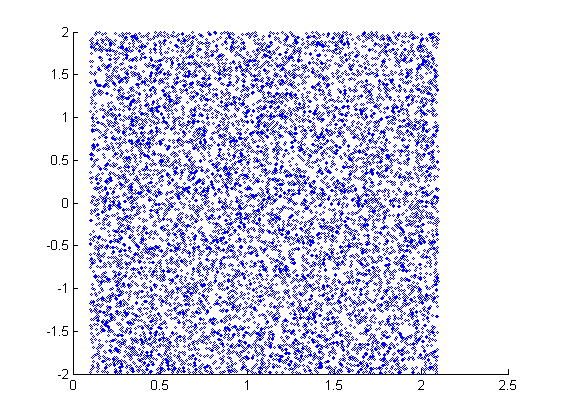
\includegraphics[width=1\textwidth]{Figs/col_m1_v1.png}
                \caption{}
                \label{fig:mom1}
        \end{subfigure}%
%
%\hspace{20mm}
\begin{subfigure}[b]{\nn\textwidth}
                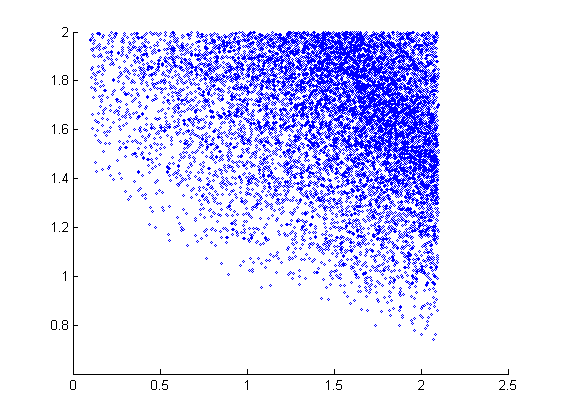
\includegraphics[width=1\textwidth]{Figs/col_m1v1_p3.png}
                \caption{}
                \label{fig:mom2}
        \end{subfigure}%
\begin{subfigure}[b]{\nn\textwidth}
                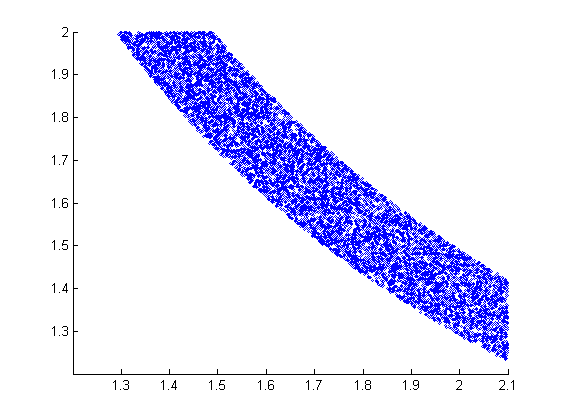
\includegraphics[width=1\textwidth]{Figs/col_m1v1_when_p_is_3_and_v2_is_0_dot_2.png}
                \caption{}
                \label{fig:mom2}
        \end{subfigure}%
\hspace{4mm}
%\\
\begin{subfigure}[b]{\nn\textwidth}
                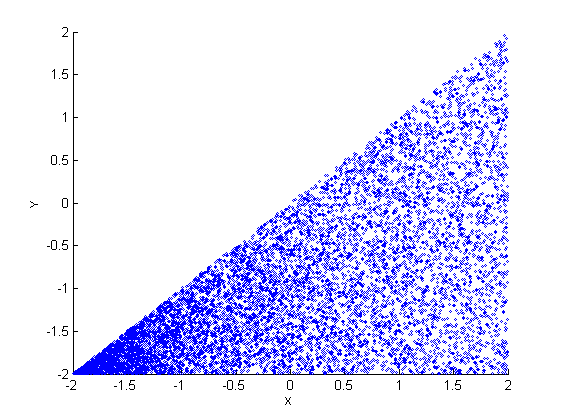
\includegraphics[width=1\textwidth]{Figs/col_v1v2.png}
                \caption{}
                \label{fig:mom2}
        \end{subfigure}%
\begin{subfigure}[b]{\nn\textwidth}
                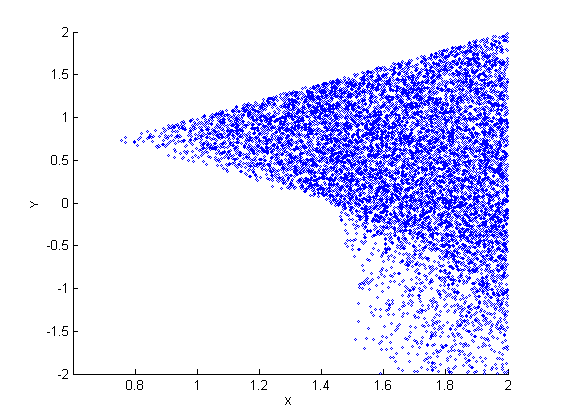
\includegraphics[width=1\textwidth]{Figs/col_v1v2whenPis3.png}
                \caption{}
                \label{fig:mom2}
        \end{subfigure}%
\begin{subfigure}[b]{\nn\textwidth}
                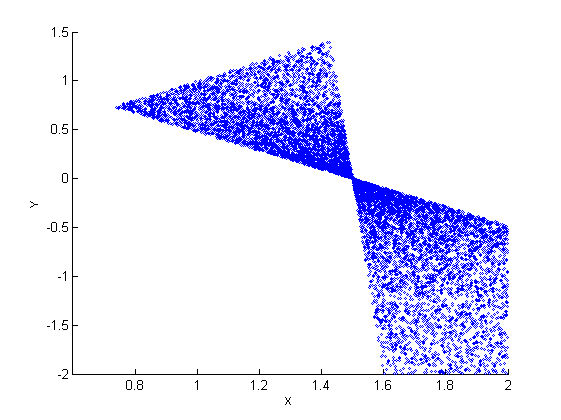
\includegraphics[width=1\textwidth]{Figs/colV1V2givenPis3M1is2.png}
                \caption{}
                \label{fig:mom2}
        \end{subfigure}%
\end{center}
\vspace{-1mm}
\caption{\footnotesize
prior/posterior joint distributions of pairs of random variables in the \emph{collision} example. 
(a) $\pr(M_1, V_1)$,
(b) $\pr(M_1, V_1 \, | \, P_3 = 3)$,
(c) $\pr(M_1, V_1 \, | \, P_3 = 3, V_2 = 0.2)$,
(d) $\pr(V_1, V_2)$,
(e) $\pr(V_1, V_2 \, | \, P_3 = 3)$,
(f) $\pr(V_1, V_2 \, | \, M_1 =2, P_3 = 3)$
} 
\label{fig:mom}
%\vspace{-4mm}
\end{figure*}



\section{Piecewise Algebraic Graphical Models}
In this section, we put things together and provide our complete model.
The requirements for the class of potential functions (factor forms) are as follows:
\begin{itemize}
\item Factor forms should be as expressive as possible to be able simulate different density forms.  
\item Factor forms should be closed under multiplication and polynomial fractional substitutions such as 
the r.h.s.\ of equation~(\ref{eq:evidence-form}). Otherwise, \emph{joint factor formation} and multiple substitutions in the \emph{collapsing determinism} phase of 
Algorithm~\ref{alg:posterior-joint} can be problematic.
\item A single analytical integration 
(i.e.\ integrating w.r.t.\ a single variable while keeping the rest of variables symbolic) should produce a closed-form structure (the requirement of Symbolic Gibbs).
\end{itemize}   

Our proposition is the use of 
the class of \emph{Polynomial-Piecewise Polynomial Fractions} (PPPFs); That is,   
functions in the form:

\begin{equation}
\label{e:ppf}
f = 
  \begin{cases}
  \case{\phi_1}{f_1}\\
\vdots\\
  \case{\phi_m}{f_m}    
  \end{cases}
\!\!\!=
  \begin{cases}
  \case{\varphi_{1,1} \lessgtr 0,\, \varphi_{1,2} \lessgtr 0,\, \ldots}{\frac{N_1}{D_1}} \\
\vdots\\
   \case{\varphi_{m,1} \lessgtr 0,\, \varphi_{m,2} \lessgtr 0,\, \ldots}{\frac{N_m}{D_m}}    
  \end{cases}
\end{equation}
where each \emph{sub-function} $f_i := \frac{N_i}{D_i}$ is a (multivariate) polynomial fraction and 
each \emph{case condition} $\phi_i$ is a conjunction of some inequalities ($\lessgtr$ stands for  
$>$ or $<$)\footnote{In piecewise distributions,  
we are careless about equalities since they only matter for $\delta[\cdot]$s which are already treated separately.} 
where each \emph{atomic constraint} $\varphi_{i,j}$ is a (multivariate) polynomial.

%Evidently, this class is very expressive. Other distributions can also be approximated by this form by being \emph{Taylor series} other existing approximation tools \cite{shenoy2011inference}.

Closure of PPPFs under multiplication is trivial, e.g.:
\begin{equation*}
\footnotesize
  \begin{cases}
  \case{\phi_1}{f_1}\\
  \case{\phi_2}{f_2}    
  \end{cases}
\,
 \otimes
\,
  \begin{cases}
  \case{\psi_1}{g_1} \\
  \case{\psi_n}{g_2} 
  \end{cases}
 \, = \,
\begin{cases}
  \case{\phi_1, \psi_1}{f_1 \times g_1} \\ 
  \case{\phi_1, \psi_2}{f_1 \times g_2} \\
  \case{\phi_2, \psi_1}{f_2 \times g_1} \\
  \case{\phi_2, \psi_2}{f_2 \times g_2}
  \end{cases}
\end{equation*} 
Closure under fractional substitution follows from the fact that 
fractional conditions can be restated as polynomials:
\begin{align*}
%\label{e:fractional2nlpa}
\left(
 \begin{cases}
  \case{\frac{F}{G} > 0}{f_1} \\ 
 \end{cases} 
\right)
 =
{\footnotesize
\begin{cases}
  \case{F > 0, G > 0 }{f_1} \\ 
  \case{F \leq 0, G \leq 0}{f_1} \\ 
 \end{cases} 
}
\end{align*}
A large group of polynomial fractions have closed-form integrals. 
We will show that this is also holds for a large group of PPPFs.
For brevity, we only focus on the following subset:

\textbf{Restricted PPPFs. }
PPPFs as in Definition~(\ref{e:ppf}) where 
each $\varphi_{i,j}$
can be written as a product of some terms $t_{i,j,k}$ where the maximum degree of each variable $X \in \bvec{X}$ in each $t_{i,j,k}$ is less or equal to 4 ($\text{rel-degree}(t_{i,j,k}) \leq 4$)
and the sub-function denominators, $D_{i}$, can be factorized into polynomials ${D}_{i,h}$ where the maximum degree of each variable in each $D_{i,h}$ is less or equal to 2 ($\text{rel-degree}(D_{i, k}) \leq 2$).%, where function $\text{rel-degree}(\cdot)$, the relative degree, is defined as follows:
 %\begin{enumerate} 
%\item Each constrain $\phi_i := \varphi_{i,1} \wedge \varphi_{i,2} \wedge \ldots$ is a conjunction of polynomial (in)equalities $\varphi_{i,j}$ such that $\text{rel-degree}(\varphi_{i,j}) \leq 4$.
%\item Each sub-function $f_i  := \frac{{N}_{i}}{{D}_{i,1} \cdot {D}_{i,2} \cdots}$
%is in the form of a fraction where the numerator ${N}_i$ 
%is an arbitrary polynomial and the denominator is factorized.
%\end{enumerate}
%\textbf{Relative degree of polynomials.} $x\text{-deg}(g)$, the degree of a polynomial $g$ w.r.t.\ a variable $x$, is the degree of $g$ if all scope variables except $x$ are considered constant. For example $x\text{-deg}(x y^2 + x^2 y z^3) = 2$. The \emph{relative degree} of $g$, $\text{rel-degree}(g)$, is:
%\[\text{rel-degree}(g) = \max_{x \in \vec{x}}(x\text{-deg}(g))\]

Here is an example of a restricted PPPF case statement:
\begin{equation*}
{\footnotesize
\singlecase{y^2-x\leq 0 \wedge x^3+2xy \geq 0}{\frac{x^2 y^3 + 7x + 10}{(5x.y^2 + 2)(y + x)^5}}
}
\end{equation*}

The class of restricted PPPFs is still quite expressive. Meanwhile restricted PPPFs have closed form (single) integrals that are not very hard to compute automatically. 

\subsection{Analytic integration of restricted PPPFs}
The space limitations do not allow us to explain the integration process in detail. 
Instead, we highlight the main issues.

Firstly, note that the definite integrals can be reduced to indefinite integrals:
{
\footnotesize
\begin{align*}
\int_{\alpha}^{\beta} f dx  = 
\int_{-\infty}^{\infty}
\left (
  \begin{cases}
  \case{x\!>\!\alpha,\, x\!<\!\beta,\, \alpha \!<\! \beta}{1}\\
 \otherwise{0}    
  \end{cases}
\otimes
  f
\right)
dx
\end{align*}
}
Secondly, note that restricted PPPFs can be restated into a form where
the degree of each variable in each atomic constraint is less or equal to 4.
For example consider a single case statement with a single atomic constraint 
$\varphi_{1,1} := t_{1,1,1} \cdot t_{1,1,2}$ (where rel-degree$(t_{1,1,k})\leq4$):
\begin{align*}
{\footnotesize
\left(
f_1 \quad \text{if } t_{1,1,1} \cdot t_{1,1,2} > 0
\right)
 =
\begin{cases}
  \case{t_{1,1,1} \!>\! 0, \, t_{1,1,2} \!>\! 0 }{f_1} \\ 
  \case{t_{1,1,1} \!\leq\! 0, \, t_{1,1,2} \!\leq\! 0 }{f_1} 
 \end{cases} 
}
\end{align*}

Thirdly, note that for each variable $x$, 
PPPFs can be transformed into piecewise structures 
in which each atomic constraint is either in form $x>L_i$ or $x<U_i$ or $I_i>0$, 
where $L_i$, $U_i$ and $I_i$ are 
algebraic expressions (not necessarily polynomials) and $x$ is not in their scope. 
%\footnote{Again, we are careless about equalities.} 
%For instance a case statement:
%\begin{align*}
%{\footnotesize
% \begin{cases}
%  \case{(xy + z) > 0 \wedge \cdots}{f_1} \\ 
%  \vdots\\
% \end{cases} \!\!\!\!\!\!=
%\begin{cases}
%  \case{(y >0) \wedge (x>\frac{z}{y}) \wedge \cdots}{f_1} \\ 
%  \case{(y <0) \wedge (x<\frac{z}{y}) \wedge \cdots}{f_1} \\ 
 % \vdots\\
% \end{cases}
%}
%\end{align*}
%Note that in the case of quadratic constraints, these transformed cases are not necessarily polynomials.
For instance for variable $x$, the case-statement in (\ref{e:single-example})
can be replaced with three cases as in (\ref{e:quadratic-trans}).
{
\footnotesize
\begin{equation}
\label{e:single-example}
\singlecase{(x^2 y + 7x^2 + x + y > 0)}{f_1}
\end{equation}
\begin{align}
\label{e:quadratic-trans}
{
\begin{cases}
  \case{(y+7>0), \, (x> -0.5 + 0.5\sqrt{1 - 4y(y+7)}) }{f_1} \\ 
  \case{(y+7>0), \, (x> -0.5 - 0.5\sqrt{1 - 4y(y+7)}) }{f_1} \\ 
  \case{(y+7<0), \, (x > -0.5 + 0.5\sqrt{1 - 4y(y+7)}),\\
& (x < -0.5 - 0.5\sqrt{1 - 4y(y+7)}) }{f_1} \\ 
 \end{cases}
}
\end{align}
}

The infinite bound integral of a case-statement 
associated with expressions with $\{L_i\}$, $\{U_i\}$ and $\{I_i\}$ 
is itself a case-statement with the same independent constraints,
a lower bound LB =$\max\{L_i\}$ and 
an upper bound UB =$ \min\{U_i\}$.
For example:
{\footnotesize 
\begin{align*}
%\footnotesize
&\int_{-\infty}^{\infty}\!\! \Big[
\singlecase{(x>3), (x>y+1), (x<y^2-7), \\
&\hspace{28mm} (-y/z > 1) , (y^2>0)}
{x^3 + xy} \Big] dx = \\
&\singlecase{(-y/z > 1) \wedge (y^2>0)}
{\Big[ \int_{\max\{3, \, y+1\}}^{y^2 - 7}x^3 + xy \Big]} 
\end{align*}  
}
What remains is to compute the indefinite integrals of sub-functions. 
The restrictions imposed on PPPF sub-functions 
guarantee that they have closed form indefinite univariate integrals.
These integrals are computed by performing polynomial division (in case needed),
followed by partial fraction decomposition and finally, using a short list of indefinite integration rules.
\begin{comment}
, integration of function~(\ref{eq:shangul}) w.r.t.\ $x$ leads to (\ref{eq:mangul}). For instance, to generate (\ref{eq:mangul}) by integrating the restricted PPPF sub-, it suffices to:
\begin{equation}
\label{eq:shangul}
\footnotesize
f_i := \frac{-x^2 y^3 + 2x y^2 -4 x y + x + y + 11}{(x+1)(x y^2 + 5)}
\end{equation}
%To compute $\int f_i \, dx$ it is sufficient consider all variables except $x$ as constants and:
\begin{equation}
\label{eq:mangul}
\footnotesize
\int f_i dx = 
-x y  + (y+2) \log (x+1) + \frac{(y+1) \log (x y^2 + 5)}{y^2}
\end{equation}
%\section{Literature review}
%\label{sec:literature}
%A bottle neck for inference in continuous/hybrid \emph{graphical models} is the integration of continuous variables required for \emph{marginalization}. The following techniques deal with this issue and provide asymptotically unbiased inference tools:\\
%{\bf Discretization.} By discretizing continuous variables, integration is approximated by summation which can be performed effectively. However, computational costs of uniform discreatization blow up exponentially in dimensionality and \emph{dynamic discretization}, as in \cite{kozlov1997nonuniform}, is an art form.The latter algorithm is in particular, problematic for random variables whose posterior marginals may vary widely w.r.t.\ different evidence for other variables \cite{cobb2006inference}.\\
%{\bf Exact solutions.}In such works, \emph{potential} functions are restricted to (or approximated with) classes of functions with closed-form integrals. A commonly used class consists of the mixture of \emph{conditional linear Gaussians (CLG)} \cite{lauritzen2001stable} However, the class of CLGs is too restrictive and many models do not fit into it. Hypercube-piecewise truncated exponentials  \cite{moral2001mixtures} (called MTEs after \emph{mixture of truncated exponentials}) form a more flexible class. Recently piecewise polynomials have attracted attention too:A method called MOP (after \emph{mixture of polynomials})consists of hypercube-piecewise polynomials \cite{shenoy2011inference} and is further generalized to hyper-rhombus-piecewise polynomials \cite{shenoy2012two}. It is shown that the family of linear piecewise polynomials is closed under integration \cite{Sanner:12} which has lead to the most flexible existing work in this family so far. Exact methods are appealing since they provide analytic solutions. However, each of them has its own shortcomings that in practice limits its use:In CLG model, discrete nodes with continuous parents are not allowed.Models based on hypercube-piecewise functions are not closed for deterministic relationships between  continuous variables and none of the mentioned models can handles nonlinear deterministic relationships.Marginalization of several variables may lead to blowup in the number of partitions and in the case of piecewise polynomials, by increasing the function degree, becomes sensible to numerical errors. \\ 
%%Piecewise polynomials are expressive and ``in theory", by using the \emph{Taylor series} any potential function can approximate by them \cite{shenoy2011inference}. However, in practice, in the case of many functions, reasonable approximations may require too many pieces or too complicated polynomial functions. On the other hand, consecutive symbolic integration operations may lead to a blow up in the number of pieces. Despite being more expressive, there are interesting applications that remain beyond the scope of the existing piecewise models.

%Because of providing closed-form, exact and analytical solutions, these methods are appealing. However, due to the short comings mentioned in Section ??? \ref{sec:literature}, their use is limited in practice.
%{\bf Sampling.}
%\\
%{\bf Our Contribution.}
\end{comment}
%%%%%%%%%%%%%%%%%%%%%%%%%%%%%%%%%%%%%%%%%

\begin{comment}
%%%%%%%%%%%%%%%%%%%%%%%%%%
\begin{figure*}
\begin{center}
%\vspace{-1mm}
\begin{subfigure}[b]{0.3\textwidth}
                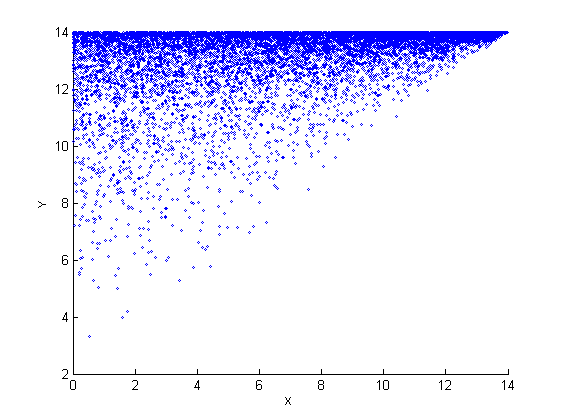
\includegraphics[width=0.7\textwidth]{Figs/alc1_AD.png}
                \caption{$\pr(A_0, A_3)$}
                \label{fig:mom1}
        \end{subfigure}%
%
%\hspace{20mm}
\begin{subfigure}[b]{0.3\textwidth}
                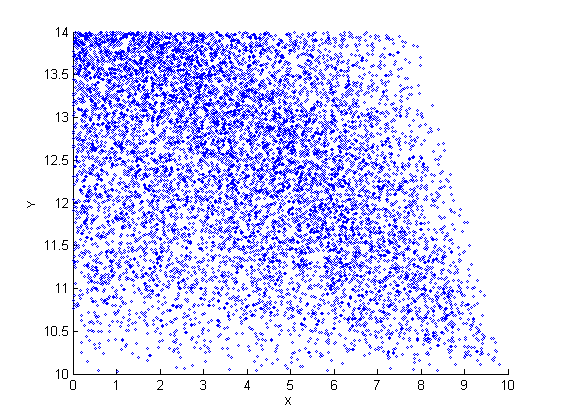
\includegraphics[width=0.7\textwidth]{Figs/alc1_ADgivenE.png}
                \caption{$\pr(A_0, A_3\,|\, (A_1 + A_2 + A_3) = 10)$}
                \label{fig:mom2}
        \end{subfigure}%
\end{center}
\vspace{-1mm}
\caption{\footnotesize 
\emph{Vintner} example.
}
\label{fig:mom}
\vspace{-4mm}
\end{figure*}
\end{comment}

%%%%%%%%%%%%%%%%%%%%%%%%%%%%%%%%%%%%%%%%%%%%%%%%%%%%%%%%
\begin{figure*}
\centering
\begin{subfigure}[b]{0.33\textwidth}
     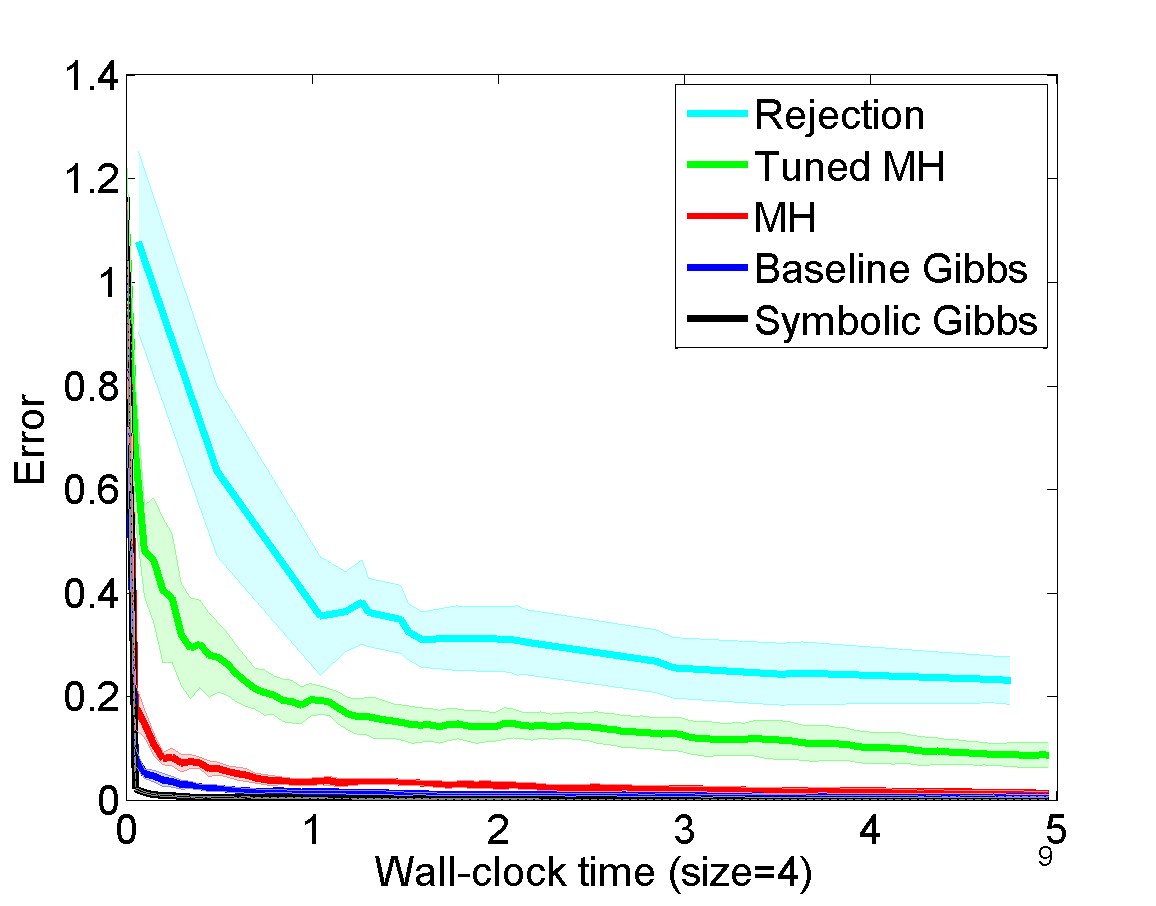
\includegraphics[width=1\linewidth, height=120pt]
{Figs/plots/collision/err-vs-time__param4-shaded.pdf}
     \caption{}
\label{fig:collision-err-vs-time4}
\end{subfigure}
%%%
\begin{subfigure}[b]{0.33\textwidth}
     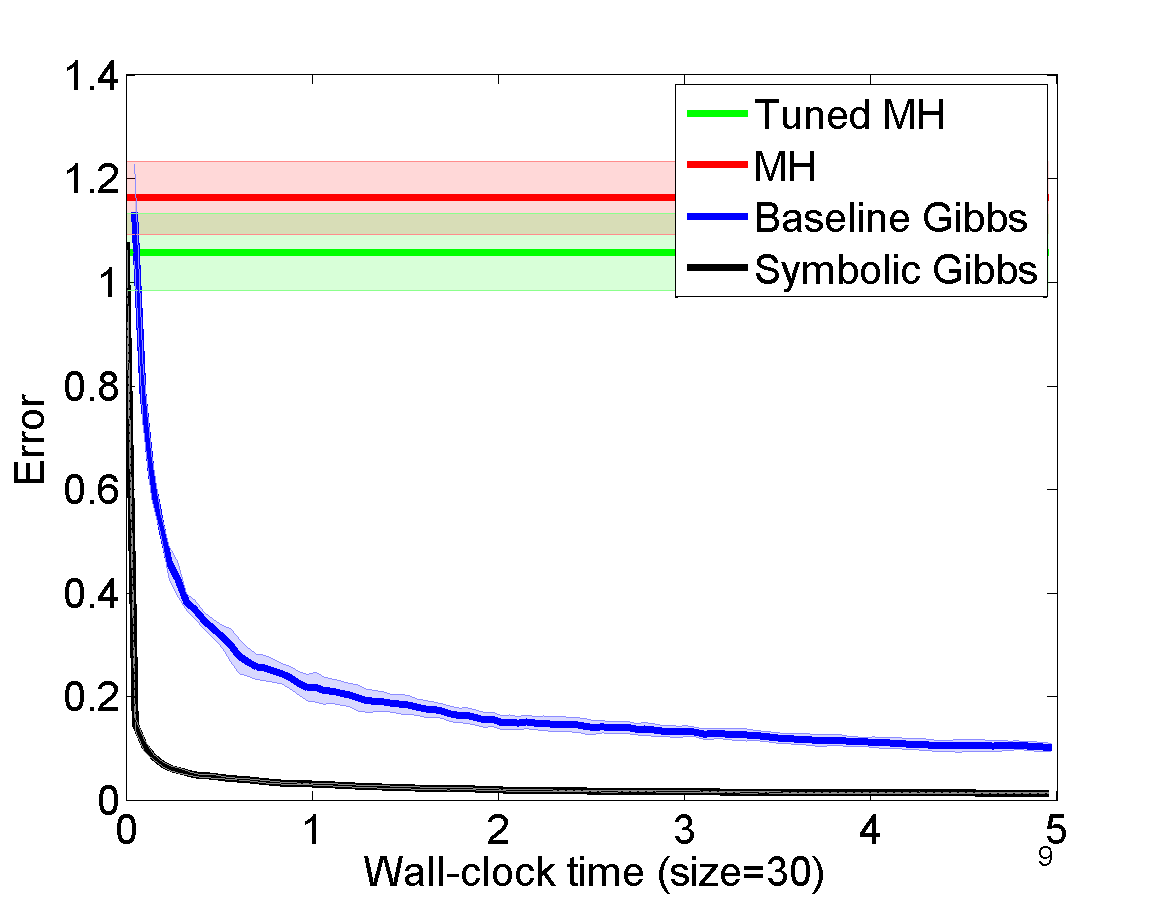
\includegraphics[width=1\linewidth, height=120pt]
{Figs/plots/collision/err-vs-time__param30-shaded.pdf}
     \caption{}
\label{fig:collision-err-vs-time30}
%\vspace{-1mm}
\end{subfigure}
\begin{minipage}[b]{0.33\textwidth}
      \caption{Error %(expected value of the difference between estimated mean vector and the ground truth vector) 
as a function of wall clock time (ns) for the generalized collision problem (Experiment 2) 
(a) for 4 colliding objects (8 stochastic variables in total since each object has a distribution over its mass and its velocity) and (b) 30 colliding objects (60 stochastic variables)
using different MCs. Note that in (b), rejection sampling has not been able to take any sample.}
      \label{fig:dummy}
    \end{minipage}
\end{figure*}
%%%%%%%%%%%%%%%%%%%%%%%%%%%%%%%%%%%%%%%%%%%%%%%%%%%%%%%%
\begin{figure*}
\begin{center}
%\vspace{-1mm}
\begin{subfigure}[b]{0.33\textwidth}
 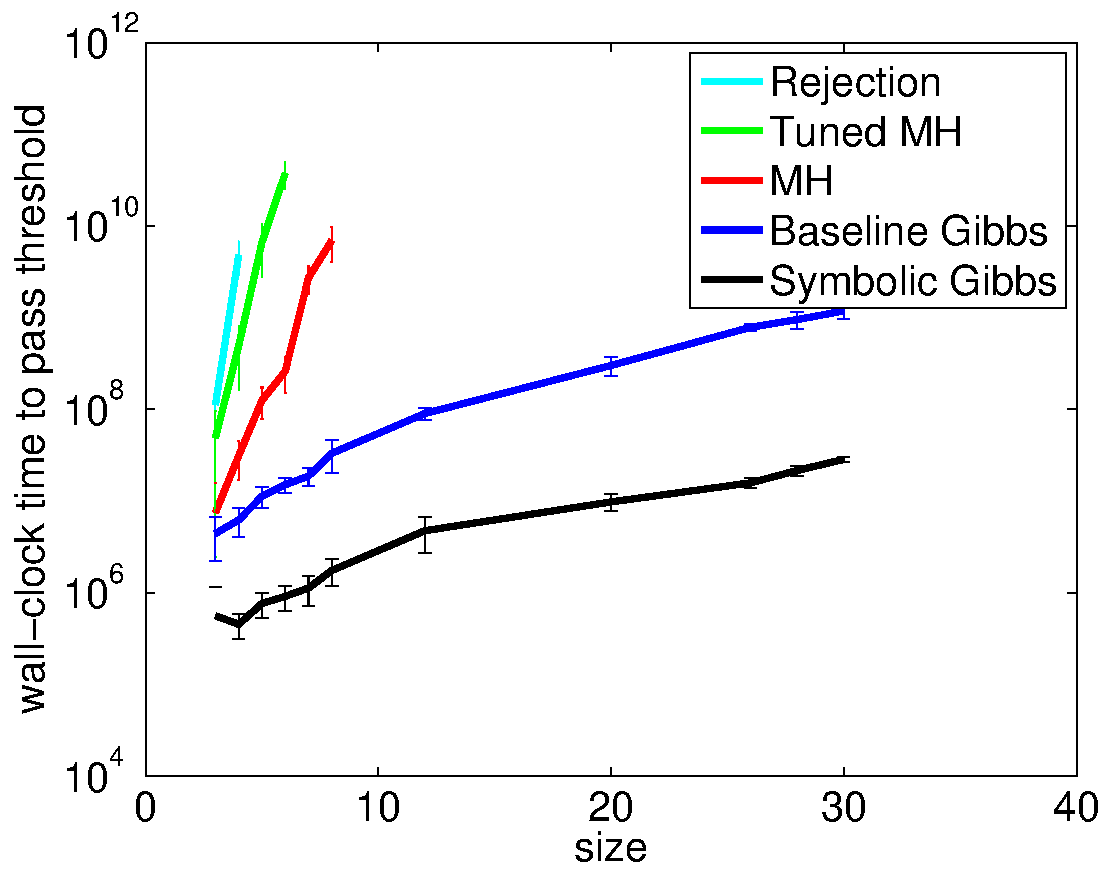
\includegraphics[width=1\linewidth, height=120pt]{Figs/plots/collision/time_vs_param-errorbar.pdf}
\caption{generalized collision problem}
\label{fig:err-threshold-vs-size-collision}
\end{subfigure}
%
\begin{subfigure}[b]{0.33\textwidth}
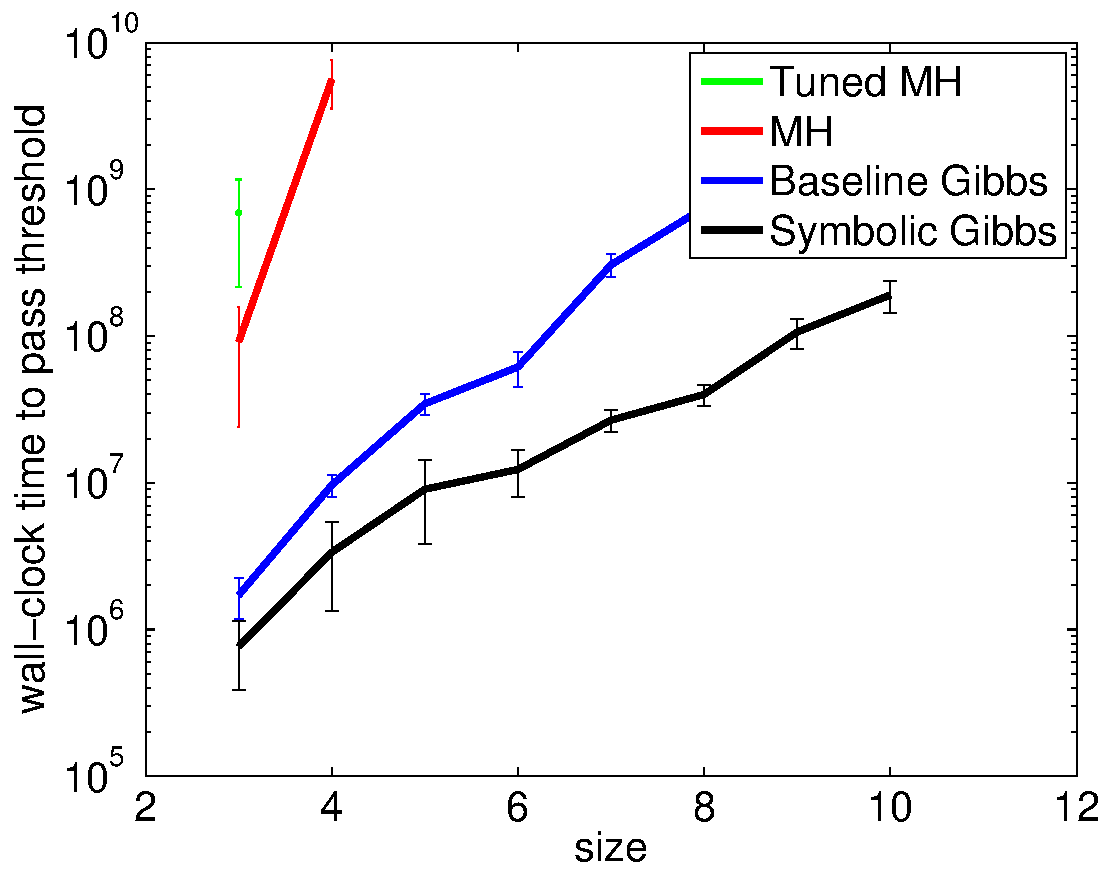
\includegraphics[width=1\linewidth, height=120pt]{Figs/plots/fermentation/time_vs_param-errorbar.pdf}
\caption{power transmission line problem}
\label{fig:err-threshold-vs-size-alc}
\end{subfigure}
\begin{subfigure}[b]{0.33\textwidth}
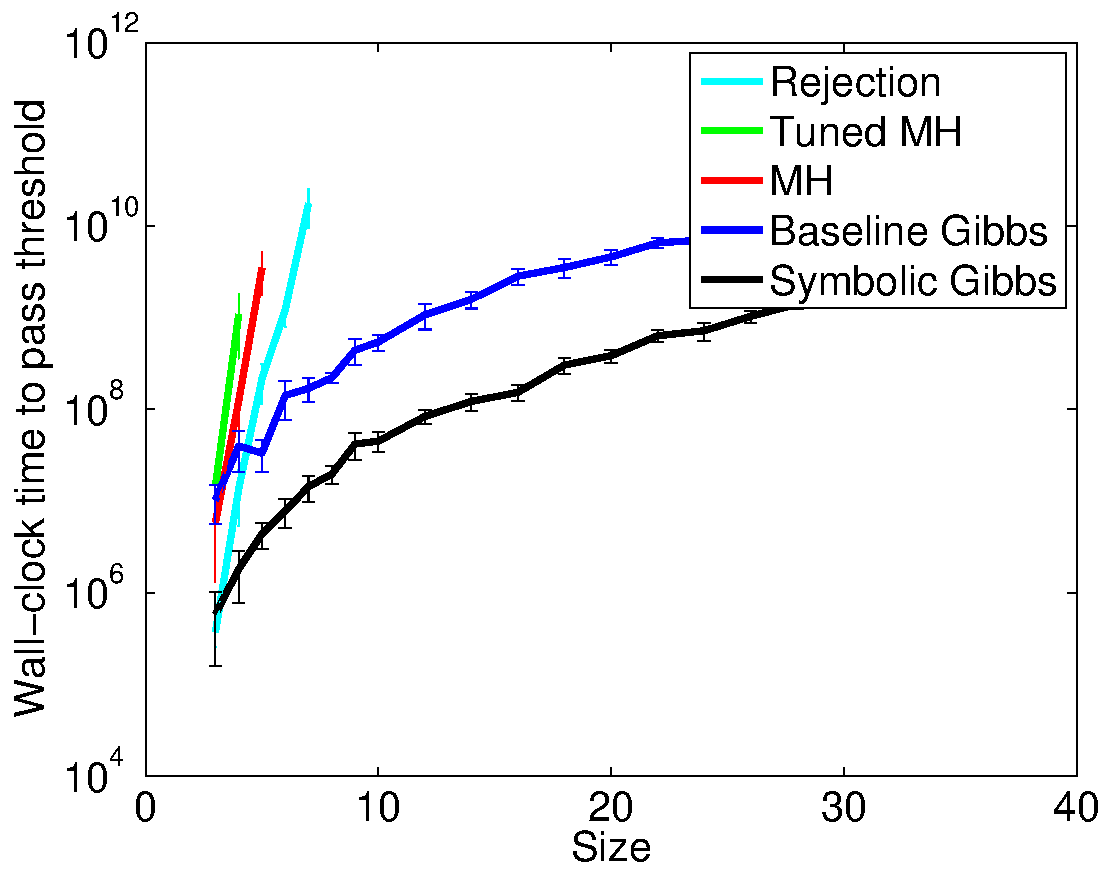
\includegraphics[width=1\linewidth, height=120pt]{Figs/plots/circuits/time_vs_param-errorbar.pdf}
\caption{reduced mass problem}
\label{fig:err-threshold-vs-size-circuit}
\end{subfigure}
\end{center}
\caption{Wall-clock time (ns) to pass a fixed error threshold vs. the GM size, for experiments 2 to 4.}
\end{figure*}

%%%%%%%%%%%%%%%%%%%%%%%%%%%%%%%%%%%%%%%%%%%%%%%%%%%%%%%%
%%%%%%%%%%%%%%%%%%%%%%%%%%%%%%%%%%%%%%%%%%%%%%%%%%%%%%%%

\section{Experimental Results}
\textbf{Experiment 1.} In our first experiment, we generate samples for the GM of the \emph{collision} example and 
plot the particles for different queries and evidence.\footnote{We have repeated the experiment for different 
MCMC methods and have made sure they generate same patterns.}
The results, as depicted in the telltale plots of Figure~\ref{fig:mom}, reveal the nature of the problem tackled in this paper.
They show that even in the presence of a single deterministic constraint, 
a simple prior can transform into a complicated posterior which is unlike any family of 
probability densities studied in the literature so far.

In the second to fourth experiments, we study the role of the size of graphical model on the performance of MCMC methods.
\\
\textbf{Experiment 2.} The second experiment is the generalization of the collision example to a case where $n$ objects 
collide. The difference is that we omit the dependency of velocities (all $V_i$ share a same uniform prior distribution) and the constraint is $\sum_i{M_i V_i} = P$. By this modification, the GM becomes symmetric and enables us to compute the true posterior mean value manually.\footnote{An alternative would be relying on \emph{MCMC convergence diagnostics} methods \cite{cowles1996markov}. The latter methods however, could produce misleading results in case MCMCs do not converge to the ground truth, a scenario that for highly complex posteriors is not improbable.} 
The tested algorithms running on the posterior are: symbolic Gibbs (ours), baseline Gibbs (CDF computation per sample), 
MH (Metropolis-Hastings tuned manually), Tuned-MH 
(automatically tuned to reach the acceptance rate of 0.234 after \cite{roberts1997weak}) and rejection sampling.
For error measure, $\mathbb{E}[|\bvec{x} - \bvec{x}^*|]$ is computed in which 
$\bvec{x}^*$ is the ground truth vector.
For each algorithm 15 Markov chains run and means and standard errors are returned.     
Figures~\ref{fig:collision-err-vs-time4} 
and 
\ref{fig:collision-err-vs-time30} 
depict error vs wall-clock time in (ns) %TODO CHECK TIME SCALE!
for a collision network of 4 and 30 objects, respectively. %(the actual number of stochastic nodes is 8 since each object is associated with a mass and velocity node).
%Figure~\ref{fig:collision-err-vs-time30} depicts the same results for 30 objects (60 nodes).
In the latter high-dimensional space, the rejection sampling has not been able to generate a particle.
MH algorithms convergence rate is very low while the baseline Gibbs still perform well and the symbolic Gibbs performance is at least an order of magnitude better.
Finally, Figure~\ref{fig:err-threshold-vs-size-collision} depicts the time to reach a fixed error threshold $T=0.2$ 
versus number of colliding objects. 
%
\\
\textbf{Experiment 3.} Here, we repeat the former experiment for a 
monotonically decreasing \emph{Dynamic Bayesian Network}. That is, a DBN with nodes $A_1$ to $A_n$
with priors: $A_1 \sim \mathcal{U}(0, b)$ and $A_t \sim \mathcal{U}(A_{t-1}, b)$ where 
$t = 2, \ldots n$ and $b=10$ is the upper bound and the deterministic constraint is $\sum A_i = c$.
This network models a power transmission line where energy loss takes place in components $A_t$.
However, many other applications, such as development of a chemical process, share similar models.  
The measurement takes place on the difference of the expected values of two parallel Markov chains to form a symmetry with ground truth \textbf{0}.
In the plotted results (Figure~\ref{fig:err-threshold-vs-size-alc}), 
the rejection sampling MC is missing since the joint is not log-concave and does not have a constant bound required for the algorithm's \emph{envelope} 
(note that $\lim_{A_{i} \rightarrow b} \frac{1}{b - A_{i}} = 0$ ).
\\
\textbf{Experiment 4.} The last experiment, with results depicted in 
Figure~\ref{fig:err-threshold-vs-size-circuit}, models an electrical circuit composed of $n$, $10\Omega\pm20\%$ paralleled resistors with bell-shaped tolerance distributions (truncated quadratics, positive in the range $[8, 12]$). The posterior tolerance distribution is computed when 
the input current $I$ and the source voltage $V$ and observed and the deterministic constraint is $\frac{1}{R_1} + \ldots + \frac{1}{R_n} = \frac{I}{V}$.
This form of equation, called \emph{reduced mass}, encounters in many problems in electrical, thermal, hydraulic, or mechanical domains. 

\section{Conclusion}

We introduced piecewise algebraic graphical models that for the first time handle a large family of nonlinear deterministic restrictions, such as the physical laws, in the form of multivariate polynomial fractions. The nonlinear nature of this data leads to a new genre of posterior distributions with possible discontinuities, 
piecewise parts with nonlinear bordering hyperplanes, rapid density changes and anomalies. Our experimental results show that Gibbs sampling performs well in the presence of such unconventional densities while other Monte Carlo methods do not. We showed that in piecewise algebraic models, the univariate CDFs required for Gibbs sampling can be computed analytically and prior to the actual sampling process. Our novel sampling method, \emph{Symbolic Gibbs}, saves a significant amount of computation, improving the performance dramatically. The combination of these novel contributions should make probabilistic reasoning applicable to variety of new applications that have remained unsolvable so far.      



%{\small
%\section*{Acknowledgements}
%NICTA is funded by the Australian Government as represented by the Department of Broadband, Communications and the Digital Economy and the Australian Research Council through the ICT Centre of Excellence program.}

\bibliography{SymbolicGibbs}
\bibliographystyle{aaai}

\end{document}
